\documentclass{beamer}

\mode<presentation>
{
  \usetheme{Warsaw}
  \setbeamercovered{transparent}
}
\usepackage[english]{babel}
\usepackage[utf8]{inputenc}
\usepackage{times}
\usepackage[T1]{fontenc}

\title[PROYECTO - ANDROID] 
{T W I T S P O L}

\subtitle
{La mejor forma de INFORMARNOS...}
\institute[ESCUELA SUPERIOR]
{	
	ESCUELA SUPERIOR\\
	POLITECNICA DEL LITORAL
}
\date[CFP 2012]{Proyecto en Android, 2012}

\begin{document}
	\begin{frame}
  	  \titlepage
	\end{frame}
	
	%Integrantes del Grupo
	\begin{frame}{INTEGRANTES}
		%\beamertemplateshadingbackground{yellow!50}{blue!50}
		 \begin{flushleft}
 			
\includegraphics[totalheight=1.2in,width=2in]{LTwitspol}
 		 \end{flushleft}
 		 
 		 \begin{itemize}
 		 	\item
 		 		\begin{flushright}
 		 			Cuadrado Daniel
 		 		\end{flushright}
 		 	\item
 		 		\begin{flushright}
 		 			Mite Juan 
 		 		\end{flushright}
 		 	\item
				\begin{flushright} 		 		
 		 		Torres Criollo Daniel
 		 		\end{flushright}
 		 	\item
 		 		\begin{flushright}
 		 			Velez Gomez José
 		 		\end{flushright}
 		 \end{itemize}
  	\end{frame}
  	
	%Resumen
	\begin{frame}{RESUMEN}
 		 \tableofcontents
  	\end{frame}
  	
  	%Seccion Introduccion
  	\section{Introduccion}
		\subsection{Vision}
		\begin{frame}{VISION DE TWITSPOL}
			\begin{block}<1->{\begin{center}{V I S I O N}\end{center}}
				\begin{center}
					El objetivo es que cada estudiante, profesor, trabajador o servidor de Espol que tenga un teléfono con 							ANDROID pueda estar informado de todos los acontecimientos de nuestra UNIVERSIDAD.
				\end{center}
			\end{block}
			
			\begin{center}
			   
\includegraphics[totalheight=1.2in,width=2in]{NTwitspol}
			\end{center}
		\end{frame}

		\subsection{Objetivos}
		\begin{frame}{OBJETIVOS ESPECIFICOS}
			\begin{itemize}[<+->]
				\item 
					Aportara al conocimiento para todos los que conformamos ESPOL.
				\item
					Se podrá recibir, crear y compartir cualquier informacion.
				\item
					Usar el MAP(Escribiendo el BLOQUE o FACULTAD) para llegar donde sea.
			\end{itemize}
			\begin{center}
				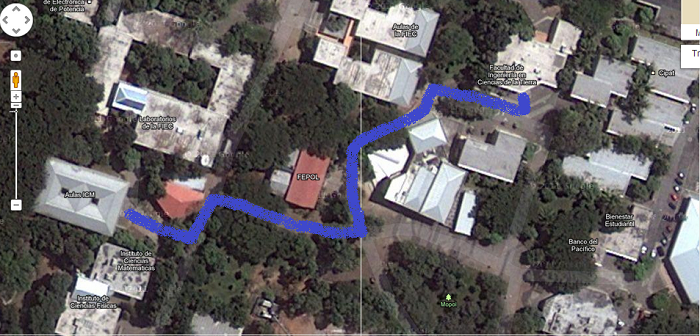
\includegraphics[totalheight=1.2in,width=4in]{Camino}
			\end{center}
		\end{frame}	

	%Seccion Contribucion	
	\section{Contribucion}
		\subsection{Servicios}
		\begin{frame}{SERVICIOS}
			\begin{itemize}[<+->]
				\item 
					Para hacer encuestas.\\
					¿Quieres enterarte de qué opinan la comunidad POLITECNICA y saber los resultados?
				\item
					Permite enviar mensajes de texto plano.
				\item
					Usar la voz para mandar mensajes.
			\end{itemize}
			\begin{center}
				
\includegraphics[totalheight=1.2in,width=4in]{TAndroid}
			\end{center}
		\end{frame}
		
		\subsection{Informaciones}		
		\begin{frame}{¿Que informaciones podemos adquirir?}
			\begin{itemize}%[<+-| alert@+>]
				\item
					DEPORTES
			\end{itemize}
			\begin{center}
				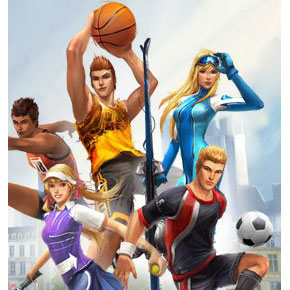
\includegraphics[totalheight=0.6in,width=0.8in]{deportes}
			\end{center}
			
			\begin{itemize}%[<+-| alert@+>]
				\item
					ACADEMICO
			\end{itemize}
			\begin{center}
				
\includegraphics[totalheight=0.6in,width=0.8in]{academico}
			\end{center}
			
			\begin{itemize}%[<+-| alert@+>]
				\item
					COMEDOR
			\end{itemize}
			\begin{center}
				
\includegraphics[totalheight=0.6in,width=0.8in]{comedor}
			\end{center}
		\end{frame}
		
		\begin{frame}
			\begin{itemize}
				\item
					TRABAJOS
			\end{itemize}
			\begin{center}
				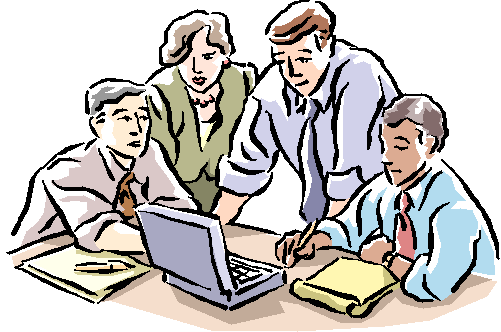
\includegraphics[totalheight=0.5in,width=1in]{trabajo}
			\end{center}						
			
			\begin{itemize}
				\item
					EVENTOS CULTURALES
			\end{itemize}
			\begin{center}
				
\includegraphics[totalheight=0.5in,width=1in]{ECulturales}
			\end{center}			
		\end{frame}
		
	%\appendix	
	\section<presentation>*{\appendixname}
	\subsection<presentation>*{TWITSPOL - ANDROID}
	\begin{frame}
	\centering
		
\includegraphics[totalheight=1.2in,width=2in]{Android}
		\begin{center}
			M U C H A S \\ G R A C I A S 
		\end{center}
	\end{frame}
	
	
\end{document}

